\documentclass{standalone}
\usepackage{tikz}
\usepackage{ctex,siunitx}
\setCJKmainfont{Noto Serif CJK SC}
\usepackage{tkz-euclide}
\usepackage{amsmath}
\usetikzlibrary{patterns, calc}
\usetikzlibrary {decorations.pathmorphing, decorations.pathreplacing, decorations.shapes,}

\begin{document}
\small
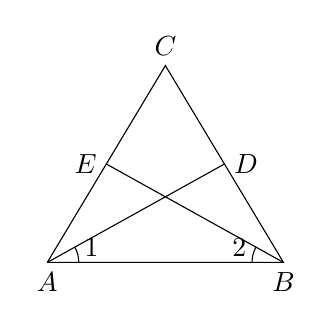
\begin{tikzpicture}[>=stealth,scale=1.0]
  \tkzSetUpPoint[fill=black]
  % \useasboundingbox(-1,-0.75)rectangle(3.7,1.4);
  \draw(-1.5,0)node[below]{$A$}--(0,2.5)node[above]{$C$}--(1.5,0)node[below]{$B$}--(-1.5,0);
  \draw(-.75,1.25)node[left]{$E$}--(1.5,0);
  \draw(.75,1.25)node[right]{$D$}--(-1.5,0);
  \draw(-1.5+.4,0) arc (0:29:.4)node[right]{1};
  \draw(1.5-.4,0) arc (180:180-29:.4)node[left]{2};
\end{tikzpicture}
\end{document}